\documentclass[10pt,a4paper]{article}
\usepackage[utf8]{inputenc}
\usepackage{amsmath}
\usepackage{amsfonts}
\usepackage{amssymb}
\usepackage{makeidx}
\usepackage{graphicx}
\usepackage[left=2cm,right=2cm,top=2cm,bottom=2cm]{geometry}
\author{Jiménez Cortés Raúl}

\begin{document}
\begin{center}
\begin{LARGE}
\textbf{INGENIERÍA MECATRÓNICA}\\
\end{LARGE}
{\large Sistemas Eletrónicos De Interfaz}\\
\begin{figure}[hbtp]
\centering

\includegraphics[scale=0.80]{UPZMG_Mecatr_nica.png}
\end{figure} 
\begin{center}
\begin{LARGE}
EV-2-3-Explicar Los Arreglos Y De Los Amplificadores Clase B.
\end{LARGE}
\end{center}

\begin{Large}
\textbf{Alumno}
\\\textit{Raúl Jiménez Cortés}
\textbf{\\Maestro}
\\\textit{Morán Garabito Carlos Enriquez}
\textbf{\\Fecha de Entrega}
\\\textit{08/10/2019}
\textbf{\\Grupo}
\\\textit{4º "B"}
\end{Large}
\end{center}

\newpage
\section{Amplificador Clase B}
Un amplificador recibe una señal de algún transductor de capacitación o de cualquier otra fuente de entrada y proporciona una versión más grande de la señal a cierto dispositivo de salida o a otra etapa de amplificación.

Un amplificador de voltaje amplificación de voltaje principalmente para incrementar voltaje de la señal de entrada, Por otro lado, los amplificadores de gran señal o de potencia, proporcionan principalmente potencia suficiente a una carga de salida para activar una bocina o algún otro dispositivo.

Es decir un amplificador de potencia es aquel que, aparte de suministrar una mayor tensión, suministran también una mayor corriente (amplificación de tensión y amplificación de corriente y, por ende, amplificación de potencia).\\
\textbf{PRINCIPIO DE FUNCIONAMIENTO DE UN AMPLIFICADOR DE POTENCIA CLASE B}\\
Un amplificador de potencia funciona en clase B cuando la polarización de dc deja al transistor casi apagado de manera que el transistor se enciende cuando a este se le aplica una señal en ac. Es decir que le transistor conducirá corriente solamente para una mitad de ciclo de la señal.

Ahora para obtener una señal de ciclo completo será necesario utilizar dos transistores y lograr que cada uno de ellos conduzca durante medios ciclos opuestos, y al tener esta operación combinada se obtiene un ciclo completo de señal de salida.

Dado que una parte del circuito "empuja" a la señal de arriba durante una mitad del ciclo y la otra parte "jala" la señal hacia abajo durante la otra mitad del ciclo, el circuito por ende se denomina de contrafase circuito push-pull.\\
\begin{center}
\begin{figure}[hbtp]
\centering
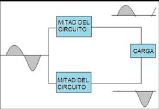
\includegraphics[scale=0.7]{1.png}
\caption{Representación En Bloques De La Operación En Contrafase.
}
\end{figure}
\end{center}
Los transistores de potencia empleados en el circuito de contrafase son capaces de entregar la potencia deseada a la carga, y la operación clase B de estos transistores proporciona una diferencia mayor que la que era posible mediante un solo transistor en la operación clase A.\\
\begin{center}
\begin{figure}[hbtp]
\centering
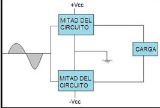
\includegraphics[scale=0.7]{2.png}
\caption{Conexión Del Amplificador En Contrafase Con La Carga Mediante Dos Fuentes De Voltaje.}
\end{figure}
\begin{figure}[hbtp]
\centering
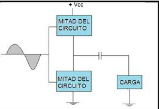
\includegraphics[scale=0.7]{3.png}
\caption{Conexión Del Amplificador En Contrafase Con La Carga Mediante Una Fuente De Voltaje.}
\end{figure}
\end{center}

\newpage
\textbf{ANALISIS EN DC}\\
\begin{center}
\begin{figure}[hbtp]
\centering
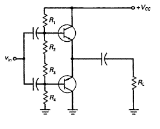
\includegraphics[scale=0.7]{4.png}
\caption{Circuito Completo }
\end{figure}
\end{center}
\begin{center}
\begin{figure}[hbtp]
\centering
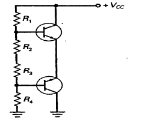
\includegraphics[scale=0.7]{5.png}
\caption{Circuito equivalente para continua}
\end{figure}
\end{center}
Con el circuito expuesto en la figura 5 se comienza el análisis en continua, el diseñador selecciona las resistencias de polarización para definir el punto Q en el corte. Esto polariza el diodo emisor de cada transistor entre 0,6 y 0,7 V de modo que estén al borde la conducción.\\
Puesto que las resistencias de polarización son iguales, cada diodo emisor se polariza con el mismo valor de tensión, como resultado, la mitad de alimentación cae en los terminales colector- emisor de cada transistor. Es decir:\\
\begin{figure}[hbtp]
\centering
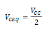
\includegraphics[scale=0.7]{6.png}
\end{figure}

\textbf{RECTA DE CARGA EN CONTINUA}\\
Debido a que no existe ninguna resistencia en los circuitos de colector ni de emisor como se observa en la figura 5, la corriente continua de saturación es infinita. Esto significa que la recta de carga continua es vertical .Lo mas complicado en el diseño de los amplificadores clase B es configurar un punto Q estable en la región de corte.\\
\textbf{RECTA DE CARGA EN ALTERNA}\\
Cuando cualquiera de los transistores esta conduciendo, su punto de operación se desplaza a lo largo de la recta de carga en alterna. La amplitud de la tensión del transistor que está en conducción puede variar entre el corte y la saturación. En el otro semiciclo, el otro transistor tendrá este mismo comportamiento. Esto significa que la salida máxima pico a pico es:  MPP=Vcc\\
\begin{center}
\begin{figure}[hbtp]
\centering
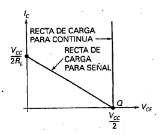
\includegraphics[scale=0.5]{7.png}
\caption{Rectas De Carga En Continua Y Alterna}
\end{figure}
\end{center}

\newpage
\textbf{ ANALISIS EN AC}\\
\begin{center}
\begin{figure}[hbtp]
\centering
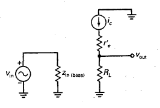
\includegraphics[scale=0.5]{8.png}
\caption{ Circuito Equivalente En Alterna}
\end{figure}
\end{center}
como se muestra en la figura 7 el circuito equivalente en alterna del transistor el mismo esta conduciendo. Ignorando re la ganancia de tensión es:\\
\begin{center}
\begin{figure}[hbtp]
\centering
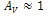
\includegraphics[scale=0.5]{9.png}
\end{figure}
\end{center}

\textbf{FUNCIONAMIENTO GLOBAL}\\\\
En el semiciclo positivo de la tensión de entrada, el transistor superior de la figura 4 conduce y el inferior esta cortado. El transistor superior se comporta como un seguidor a emisor normal, por lo que la tensión de salida es aproximadamente igual a la tensión de entrada.
En el semiciclo negativo de la tensión de entrada, el transistor superior está cortado y el transistor inferior conduce. El transistor inferior se comporta como un seguidor de emisor normal y produce una tensión de carga aproximadamente igual a la tensión de entrada. El transistor superior maneja el semiciclo positivo de la tensión de entrada y el transistor inferior se ocupa del semiciclo negativo. Durante cada semiciclo, la fuente ve una alta impedancia en cualquiera de las bases.\\\\
\newpage
\textbf{POTENCIA DE ENTRADA (dc)}\\
La potencia proporcionada a la carga por un amplificador se toma de la fuente de alimentación (o fuentes de alimentación) que proporciona la potencia de entrada de dc. La cantidad de esta potencia de entrada puede ser calculada mediante:\\
\begin{center}
\begin{figure}[hbtp]
\centering
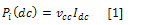
\includegraphics[scale=0.5]{11.png}
\end{figure}
\end{center}
Donde:\\

\begin{center}
\begin{figure}[hbtp]
\centering
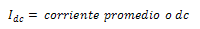
\includegraphics[scale=0.5]{12.png}
\end{figure}
\end{center}
Se consume de las fuentes de alimentación. En la operación clase B, el consumo de corriente de una sola fuente de alimentación tiene la forma de una señal rectificada de onda completa, mientras que la extraída de dos fuentes de alimentación tiene la forma de una señal rectificada demedia onda de cada fuente. Donde el valor promedio de la corriente puede expresarse de la siguiente manera.\\

\begin{center}
\begin{figure}[hbtp]
\centering
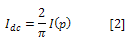
\includegraphics[scale=0.5]{13.png}
\end{figure}
\end{center}

Donde:\\
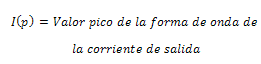
\includegraphics[scale=0.5]{14.png} 

Al utilizar la ecuación [2] en la ecuación de potencia de entrada [1] se obtiene:\\
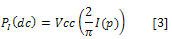
\includegraphics[scale=0.5]{15.png} 

\textbf{POTENCIA DE SALIDA (ac)}\\
La potencia aplicada a la carga (referida comúnmente como una resistencia Monografias.comse puede calcular mediante cualquiera de distintas ecuaciones. Si se utiliza un medidor rms para medir el voltaje a través de la carga, la potencia de salida se puede calcular como:\\
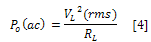
\includegraphics[scale=0.5]{16.png} 

\textbf{EFICIENCIA}\\
La eficiencia del amplificador clase B puede calcularse mediante la ecuación básica:\\
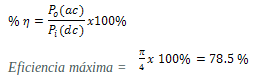
\includegraphics[scale=0.5]{17.png}

\textbf{ POTENCIA DISIPADA POR LOS TRANSISTORES DE SALIDA}\\
La potencia disipada en forma de calor por los transistores de potencia de salida será la diferencia entre la potencia de entrada aplicada por las fuentes y la potencia de salida aplicada a la carga.\\
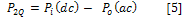
\includegraphics[scale=0.5]{18.png}

Donde:\\
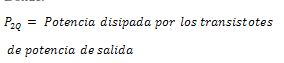
\includegraphics[scale=0.5]{19.png}

\textbf{CIRCUITO AMPLIFICADOR CLASE B}\\
Es posible obtener la clase B mediante arreglos de circuitos. Ahora se analizaran las ventajas y las desventajas de algunos de los circuitos más comunes. Las señales de entrada del amplificador pueden ser una sola señal, que luego se proporciona a un circuito con dos etapas de salida diferentes, de las cuales cada una opera durante una mitad del ciclo. Si la entrada se encuentra en la forma de dos señales de polaridad opuesta, pueden emplearse dos etapas similares, de las cuales cada una ópera sobre el ciclo alterno debido a la señal de entrada.\\
\begin{center}
\begin{figure}[hbtp]
\centering
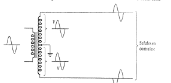
\includegraphics[scale=0.5]{20.png}
\caption{Forma De Obtener Una Señal Con Fase Invertida}
\end{figure}
\end{center}

Una forma para obtener inversión de polaridad o de fase es mediante el uso de transformadores, entre los que es muy popular desde hace mucho tiempo el amplificador acoplado por transformador. También es posible obtener una operación con polaridad opuesta al utilizar una sola entrada y transistores complementarios.\\
\textbf{CIRCUITOS EN CONTRAFASE ACOPLADOS POR TRANSFORMADOR}\\
\begin{center}
\begin{figure}[hbtp]
\centering
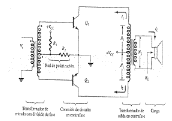
\includegraphics[scale=0.5]{21.png}
\caption{ Circuito Simétrico En Contrafase.}
\end{figure}
\end{center}

El circuito de la figura 4 emplea un transformador de entrada con derivación central para producir señales de polaridad opuesta a las dos entradas del transistor y un transformador de salida para accionar la carga en un modo de operación en contrafase que se describe de la siguiente manera:

Durante la primera mitad del ciclo de operación, El transistor Q1 se activa para conducir mientras que el transistor Q2 se desactiva. La corriente I1 que pasa a través del transformador da como resultado el primer medio ciclo de la señal a la carga. Durante el segundo medio ciclo de la señal de entrada Q2 conduce mientras Q1 permanece apagado. La corriente I2 a través del transformador da como resultado el segundo medio ciclo a la carga. La señal total generada a través de la carga entonces variara durante el ciclo completo de la operación de la señal.\\
\textbf{CIRCUITOS SIMETRICOS COMPLEMENTARIOS}\\
Al utilizar transistores complementarios (npn y pnp) es posible obtener una salida de ciclo completo a través de una carga mediante medios ciclos de operación de cada transistor.\\
\begin{center}
\begin{figure}[hbtp]
\centering
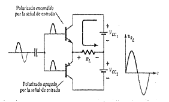
\includegraphics[scale=0.5]{22.png}
\caption{Salida De Ciclo Completo A Través De Una Carga}
\end{figure}
\end{center}

Mientras se aplica una señal sencilla de entrada a la base de ambos transistores, que son de tipo opuesto, conducirán en medios ciclos opuestos de la entrada. El transistor npn se polarizara para conducir por el medio ciclo positivo de la señal, con un medio ciclo de señal resultante a través de la carga. Durante el medio ciclo negativo de la señal, el transistor pnp se polarizara para conducir cuando la entrada se vuelva negativa.

Durante un ciclo completo de la entrada, se desarrollara un ciclo completo de señal de entrada a través de la carga. Una desventaja del circuito es la necesidad de dos fuentes de alimentación de voltaje separadas. Otra desventaja menos obvia, con el circuito complementario se observa en la distorsión de cruce o transición resultante en la señal de entrada.

La distorsión de cruce se refiere al hecho de que durante la transición de la señal de positiva a negativa (o viceversa) existe una cierta no linealidad en la señal de salida.\\
\begin{center}
\begin{figure}[hbtp]
\centering
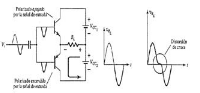
\includegraphics[scale=0.5]{23.png}
\caption{Salida De Ciclo Completo A Través De Una Carga Y La Distorsión De Cruce.}
\end{figure}
\end{center}

\begin{center}
\begin{figure}[hbtp]
\centering
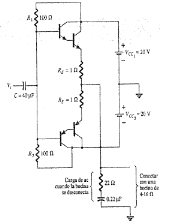
\includegraphics[scale=0.5]{24.png}
\caption{Salida En Contrafase Mediante Transistores Complementarios. (DARLINGTON)}
\end{figure}
\end{center}
En la figura anterior se observa que la carga se maneja como la salida de un emisor -seguidor de forma que la resistencia de carga de la carga es igualada por la baja resistencia de salida de la fuente excitadora. El circuito usa transistores complementarios conectados en Darlington para proporcionar una corriente mayor de salida y una menor resistencia de salida.\\
\textbf{AMPLIFICADOR EN CONTRAFASE CAUSICOMPLEMENTARIO}\\
En los amplificadores de potencia prácticos, es preferible usar transistores npn para ambos dispositivos de lata corriente de salida. Debido a que la conexión en contrafase requiere dispositivos complementarios, se deberá utilizar un transistor pnp de alta potencia. Un medio practico de obtener una operación complementaria mientras se utilizan los mismos transistores npn acoplados a la salida, lo ofrece un circuito causicomplementario. Como se muestra en la figura 13.
\begin{center}
\begin{figure}[hbtp]
\centering
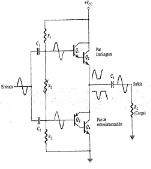
\includegraphics[scale=0.5]{25.png}
\caption{Amplificador De Potencia En Contrafase Causicomplementario Sin Transformador.}
\end{figure}
\end{center}
La operación en contrafase se logra mediante el uso de transistores complementarios Q1 y Q2 antes de los transistores npn de salida acoplados Q3 y Q4. Se observa que los transistores Q1 y Q3 forman una conexión Darlington que proporcionan la salida de un emisor seguidor de baja impedancia. La conexión de los transistores Q2 y Q4 forma un par retroalimentado, el cual, de forma similar, proporcionan un manejo de baja impedancia para la carga .El resistor R2 se puede ajustar para minimizar la distorsión de cruce mediante el ajuste de la condición de polarización de dc. L a señal única de de entrada aplicada a la etapa de contrafase, entonces ocasiona una salida de ciclo completo para la carga. El amplificador en contrafase causicomplementrario es actualmente la forma mas popular de amplificador de potencia.\\

\section{Referencias}
Boylestad Nashelsky, Electronica teoría de circuitos y dispositivos electrónicos, editorial Perason, 8va edición , Pag 761-769.

Albert Malvino, Principios de electrónica, editorial Mc Graw Hill ,6ta edición , Pag 395.


\bibliography{Tarea4.bib}{https://www.monografias.com/trabajos89/amplificador-potencia-clase-b/amplificador-potencia-clase-b.shtml}
\bibliographystyle{plain}
\end{document}